% f2015zjl_q05_parabola.tex — 2015 年高考数学·浙江卷·理科 第 5 题（抛物线与三点）
%
% 【来源】`.work/phase3-b19/source/2015浙江理.pdf`（SHA-256
%   801150f0a6d440ac967813d264face6d48b6ee9c69cc20f1c9d6b2b38dec2e9f），
%   第 1 页（合订本页 989）；内容对象 5。逐路径实测见
%   `.work/phase3-b19/figure-inventory.md`。
%
% 【坐标口径】源 PDF 用户空间（原点左下、y 向上）。本图本地坐标
%   (x, y) = (x_page − 509.212, y_page − 599.834)，1 单位 = 1 TeX pt。
%   路径坐标逐点照录内容流（含三次贝塞尔控制点）。
%
% 元素计数：10 条路径（x/y 轴＋箭头、上下两支抛物线、割线 C–B–A、CF/FB/FA）＋7 个标签
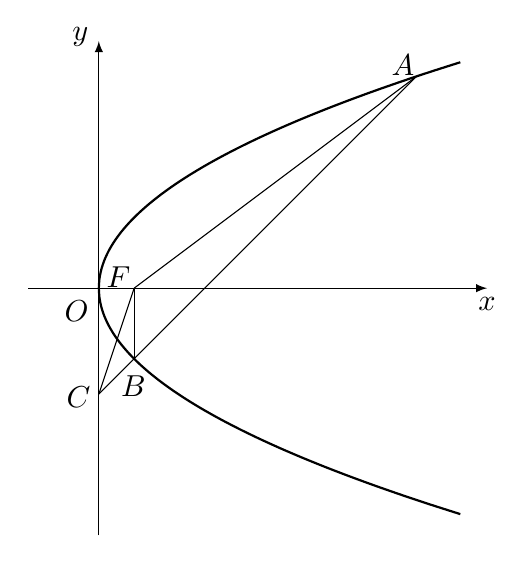
\begin{tikzpicture}[x=1pt, y=1pt,
    every node/.style={inner sep=0pt, font=\fontsize{10.5pt}{12.6pt}\selectfont}]
  \draw[line width=0.398pt] (0.0001,89.2920)   -- (162.2411,89.2920);
  \fill[line width=1.0pt] (165.8277,89.2920)   .. controls (164.7647,89.4910) and (163.0377,90.0890) .. (161.8427,90.7860)   -- (161.8427,87.7980)   .. controls (163.0377,88.4950) and (164.7647,89.0930) .. (165.8277,89.2920);
  \draw[line width=0.398pt] (25.5120,0.0002)   -- (25.5120,174.9972);
  \fill[line width=1.0pt] (25.5120,178.5838)   .. controls (25.3130,177.5208) and (24.7150,175.7938) .. (24.0180,174.5988)   -- (27.0060,174.5988)   .. controls (26.3090,175.7938) and (25.7110,177.5208) .. (25.5120,178.5838);
  \draw[line width=0.797pt] (25.5120,89.2920)   .. controls (25.5120,89.2920) and (25.6130,91.7500) .. (25.7390,92.6940)   .. controls (25.8650,93.6370) and (26.1670,95.1510) .. (26.4190,96.0950)   .. controls (26.6710,97.0390) and (27.1750,98.5530) .. (27.5530,99.4970)   .. controls (27.9300,100.4410) and (28.6370,101.9540) .. (29.1400,102.8980)   .. controls (29.6440,103.8420) and (30.5520,105.3560) .. (31.1810,106.3000)   .. controls (31.8100,107.2440) and (32.9200,108.7570) .. (33.6750,109.7010)   .. controls (34.4310,110.6450) and (35.7420,112.1590) .. (36.6230,113.1030)   .. controls (37.5040,114.0470) and (39.0180,115.5600) .. (40.0250,116.5040)   .. controls (41.0320,117.4480) and (42.7470,118.9620) .. (43.8800,119.9060)   .. controls (45.0120,120.8500) and (46.9300,122.3630) .. (48.1880,123.3070)   .. controls (49.4470,124.2510) and (51.5660,125.7650) .. (52.9500,126.7090)   .. controls (54.3350,127.6530) and (56.6560,129.1670) .. (58.1660,130.1110)   .. controls (59.6770,131.0540) and (62.1990,132.5680) .. (63.8350,133.5120)   .. controls (65.4710,134.4560) and (68.1960,135.9700) .. (69.9580,136.9140)   .. controls (71.7200,137.8570) and (74.6470,139.3710) .. (76.5340,140.3150)   .. controls (78.4220,141.2590) and (81.5500,142.7730) .. (83.5640,143.7170)   .. controls (85.5780,144.6610) and (88.9080,146.1740) .. (91.0470,147.1180)   .. controls (93.1870,148.0620) and (96.7190,149.5760) .. (98.9840,150.5200)   .. controls (101.2490,151.4640) and (104.9830,152.9770) .. (107.3740,153.9210)   .. controls (109.7660,154.8650) and (113.7010,156.3790) .. (116.2180,157.3230)   .. controls (118.7350,158.2670) and (122.8730,159.7800) .. (125.5160,160.7240)   .. controls (128.1590,161.6680) and (132.4980,163.1820) .. (135.2670,164.1260)   .. controls (138.0350,165.0700) and (142.5760,166.5840) .. (145.4710,167.5270)   .. controls (148.3660,168.4710) and (156.1290,170.9290) .. (156.1290,170.9290);
  \draw[line width=0.797pt] (25.5120,89.2920)   .. controls (25.5120,89.2920) and (25.6130,86.8340) .. (25.7390,85.8900)   .. controls (25.8650,84.9470) and (26.1670,83.4330) .. (26.4190,82.4890)   .. controls (26.6710,81.5450) and (27.1750,80.0310) .. (27.5530,79.0870)   .. controls (27.9300,78.1430) and (28.6370,76.6300) .. (29.1400,75.6860)   .. controls (29.6440,74.7420) and (30.5520,73.2280) .. (31.1810,72.2840)   .. controls (31.8100,71.3400) and (32.9200,69.8270) .. (33.6750,68.8830)   .. controls (34.4310,67.9390) and (35.7420,66.4250) .. (36.6230,65.4810)   .. controls (37.5040,64.5370) and (39.0180,63.0240) .. (40.0250,62.0800)   .. controls (41.0320,61.1360) and (42.7470,59.6220) .. (43.8800,58.6780)   .. controls (45.0120,57.7340) and (46.9300,56.2210) .. (48.1880,55.2770)   .. controls (49.4470,54.3330) and (51.5660,52.8190) .. (52.9500,51.8750)   .. controls (54.3350,50.9310) and (56.6560,49.4170) .. (58.1660,48.4730)   .. controls (59.6770,47.5300) and (62.1990,46.0160) .. (63.8350,45.0720)   .. controls (65.4710,44.1280) and (68.1960,42.6140) .. (69.9580,41.6700)   .. controls (71.7200,40.7270) and (74.6470,39.2130) .. (76.5340,38.2690)   .. controls (78.4220,37.3250) and (81.5500,35.8110) .. (83.5640,34.8670)   .. controls (85.5780,33.9230) and (88.9080,32.4100) .. (91.0470,31.4660)   .. controls (93.1870,30.5220) and (96.7190,29.0080) .. (98.9840,28.0640)   .. controls (101.2490,27.1200) and (104.9830,25.6070) .. (107.3740,24.6630)   .. controls (109.7660,23.7190) and (113.7010,22.2050) .. (116.2180,21.2610)   .. controls (118.7350,20.3170) and (122.8730,18.8040) .. (125.5160,17.8600)   .. controls (128.1590,16.9160) and (132.4980,15.4020) .. (135.2670,14.4580)   .. controls (138.0350,13.5140) and (142.5760,12.0000) .. (145.4710,11.0570)   .. controls (148.3660,10.1130) and (156.1290,7.6550) .. (156.1290,7.6550);
  \draw[line width=0.398pt] (25.5120,51.0241)   .. controls (25.5120,51.0241) and (28.9680,54.4801) .. (30.2950,55.8071)   .. controls (31.6230,57.1351) and (33.7520,59.2641) .. (35.0790,60.5911)   .. controls (36.4060,61.9181) and (38.5350,64.0471) .. (39.8620,65.3741)   .. controls (41.1900,66.7021) and (43.3190,68.8311) .. (44.6460,70.1581)   .. controls (45.9730,71.4851) and (48.1020,73.6141) .. (49.4290,74.9411)   .. controls (50.7570,76.2691) and (52.8860,78.3981) .. (54.2130,79.7251)   .. controls (55.5400,81.0521) and (57.6690,83.1811) .. (58.9960,84.5081)   .. controls (60.3240,85.8361) and (62.4530,87.9651) .. (63.7800,89.2921)   .. controls (65.1070,90.6191) and (67.2360,92.7481) .. (68.5630,94.0751)   .. controls (69.8910,95.4031) and (72.0190,97.5311) .. (73.3470,98.8591)   .. controls (74.6740,100.1861) and (76.8030,102.3151) .. (78.1300,103.6421)   .. controls (79.4580,104.9701) and (81.5860,107.0981) .. (82.9140,108.4261)   .. controls (84.2410,109.7531) and (86.3700,111.8821) .. (87.6970,113.2091)   .. controls (89.0250,114.5371) and (91.1530,116.6651) .. (92.4810,117.9931)   .. controls (93.8080,119.3201) and (95.9370,121.4491) .. (97.2640,122.7761)   .. controls (98.5920,124.1041) and (100.7200,126.2321) .. (102.0480,127.5601)   .. controls (103.3750,128.8871) and (105.5040,131.0161) .. (106.8310,132.3431)   .. controls (108.1590,133.6711) and (110.2870,135.7991) .. (111.6150,137.1271)   .. controls (112.9420,138.4541) and (115.0710,140.5831) .. (116.3980,141.9101)   .. controls (117.7260,143.2381) and (119.8540,145.3661) .. (121.1820,146.6941)   .. controls (122.5090,148.0211) and (124.6380,150.1501) .. (125.9650,151.4771)   .. controls (127.2930,152.8051) and (129.4210,154.9331) .. (130.7490,156.2611)   .. controls (132.0760,157.5881) and (134.2050,159.7171) .. (135.5320,161.0441)   .. controls (136.8600,162.3721) and (140.3160,165.8281) .. (140.3160,165.8281);
  \draw[line width=0.398pt] (38.2680,89.2920)   -- (140.3160,165.8280);
  \draw[line width=0.398pt] (38.2680,89.2920)   -- (38.2680,63.7800);
  \draw[line width=0.398pt] (25.5120,51.0240)   -- (38.2680,89.2920);

  \node[anchor=center] at (18.838,180.006) {$y$};  % 源中心 (528.05,779.84)
  \node[anchor=center] at (135.388,169.806) {$A$};  % 源中心 (644.60,769.64)
  \node[anchor=center] at (32.588,93.256) {$F$};  % 源中心 (541.80,693.09)
  \node[anchor=center] at (165.788,83.706) {$x$};  % 源中心 (675.00,683.54)
  \node[anchor=center] at (17.488,81.006) {$O$};  % 源中心 (526.70,680.84)
  \node[anchor=center] at (18.138,50.056) {$C$};  % 源中心 (527.35,649.89)
  \node[anchor=center] at (37.988,53.856) {$B$};  % 源中心 (547.20,653.69)

\end{tikzpicture}
%
% 【自验结果】
%   探针：latexmk -pdfxe（待跑）。
